\documentclass[11pt]{article} 

\usepackage[utf8]{inputenc} 

%%% PAGE DIMENSIONS
\usepackage{geometry} % to change the page dimensions
\geometry{a4paper} % or letterpaper (US) or a5paper or....
\geometry{margin=1in} % for example, change the margins to 2 inches all round

\usepackage{graphicx} % support the \includegraphics command and options

%%% PACKAGES
\usepackage{booktabs} % for much better looking tables
\usepackage{array} % for better arrays (eg matrices) in maths
\usepackage{paralist} % very flexible & customisable lists (eg. enumerate/itemize, etc.)
\usepackage{verbatim} % adds environment for commenting out blocks of text & for better verbatim
%\usepackage{subfig} % make it possible to include more than one captioned figure/table in a single float
\usepackage{enumitem}
\usepackage{multicol}
\usepackage{tikz}
\usepackage{subcaption}
\usepackage{multirow}
\usepackage[brazilian]{babel}
\usepackage{circuitikz}
\tikzset{
  declare function={% in case of CVS which switches the arguments of atan2
    atan3(\a,\b)=ifthenelse(atan2(0,1)==90, atan2(\a,\b), atan2(\b,\a));},
  kinky cross radius/.initial=+.125cm,
  @kinky cross/.initial=+, kinky crosses/.is choice,
  kinky crosses/left/.style={@kinky cross=-},kinky crosses/right/.style={@kinky cross=+},
  kinky cross/.style args={(#1)--(#2)}{
    to path={
      let \p{@kc@}=($(\tikztotarget)-(\tikztostart)$),
          \n{@kc@}={atan3(\p{@kc@})+180} in
      -- ($(intersection of \tikztostart--{\tikztotarget} and #1--#2)!%
             \pgfkeysvalueof{/tikz/kinky cross radius}!(\tikztostart)$)
      arc [ radius     =\pgfkeysvalueof{/tikz/kinky cross radius},
            start angle=\n{@kc@},
            delta angle=\pgfkeysvalueof{/tikz/@kinky cross}180 ]
      -- (\tikztotarget)}}}

%%% HEADERS & FOOTERS
\usepackage{fancyhdr} % This should be set AFTER setting up the page geometry
\pagestyle{fancy} % options: empty , plain , fancy
\renewcommand{\headrulewidth}{0pt} % customise the layout...
\lhead{}\chead{Universidade Federal Fluminense\\Departamento de Engenharia Elétrica\\TEE00129 - Laboratório de Eletrônica Básica}\rhead{}
\lfoot{}\cfoot{\thepage}\rfoot{}

%%% SECTION TITLE APPEARANCE
%\usepackage{sectsty}
%\allsectionsfont{\sffamily\mdseries\upshape} % (See the fntguide.pdf for font help)

%%% ToC (table of contents) APPEARANCE
\usepackage[nottoc,notlof,notlot]{tocbibind} % Put the bibliography in the ToC
\usepackage[titles,subfigure]{tocloft} % Alter the style of the Table of Contents
\renewcommand{\cftsecfont}{\rmfamily\mdseries\upshape}
\renewcommand{\cftsecpagefont}{\rmfamily\mdseries\upshape} % No bold!

%%% END Article customizations

\title{Aula 3: Retificadores de Onda Completa}
\author{Prof. Derick Furquim Pereira}
\date{} % Activate to display a given date or no date (if empty),
         % otherwise the current date is printed 

\begin{document}
\maketitle
\thispagestyle{fancy}

\section*{Parte teórica}

\subsection*{Questionário}

\begin{enumerate}

\item (3,0 pontos) Dado o circuito abaixo, onde $v_i(t)=V_P\sin\omega t$, esboce a forma de onda de $v_o(t)$ e no mesmo gráfico indique em quais momentos cada um dos diferentes diodos entra em condução. Por fim, calcule o valor médio de $v_o(t)$.

\begin{figure}[!h]
	\centering
	\begin{circuitikz}[american voltages,scale=.7, transform shape]
		\draw (0,-.25) to[open, v=$v_i(t)$] (3,-.25);
		\draw (3,0) to[sV, *-*] (0,0);
		\draw (0,0) to[Do, l=$D_1$] (0,3);
		\draw (3,0) to[Do, l=$D_2$, -*] (3,3);
		\draw (0,-3) to[Do, l=$D_3$] (0,0);
		\draw (3,-3) to[Do, l=$D_4$, *-] (3,0);
		\draw (0,3) to[short] (5,3);
		\draw (0,-3) to[short] (5,-3);
		\draw (5,3) to[R, l_=$R$,-*] (5,-3);
		\draw (5,1.5) to[open, v^=$v_o(t)$] (5,-1.5);
		\draw (5,-3) node[ground] {};
	\end{circuitikz}
\end{figure}

\item (1,0 pontos) Com base na resposta da questão anterior, responda:

\begin{enumerate}
\item Qual a relação entre as frequências de $v_o$ e $v_i$? Justifique.
\item A tensão de saída $v_o$ é contínua? Justifique.
\end{enumerate}

\end{enumerate}

\section*{Retificador de onda completa com derivação central}

\subsection*{Procedimento}

Coloque a chave S1 do \textit{DIP Switch} na posição fechada (ON) e mantenha as demais chaves na posição aberta. Nesta condição, tem-se o circuito equivalente mostrado na Figura \ref{circ1}.

\begin{figure}[!htb]
\centering
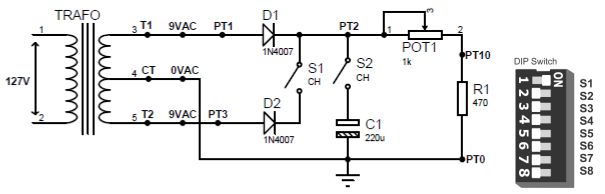
\includegraphics[width=.7\textwidth]{RetificadorOndaCompleta.png}
\caption{Circuito equivalente do retificador de onda completa com derivação central.}
\label{circ1}
\end{figure}

Para realizar a filtragem capacitiva da tensão na saída do retificador da Figura \ref{circ1}, posicione as chaves S1 e S2 do \textit{DIP Switch} na posição fechada (ON) e mantenha as demais abertas. Desta forma, o capacitor C1 da Figura \ref{circ1} é inserido na saída do retificador.

\subsection*{Questionário}

\begin{enumerate}
\setcounter{enumi}{2}
\item (2,0 pontos) Com o auxílio de um osciloscópio, meça a tensão de saída do retificador de onda completa (Figura \ref{circ1}) \textbf{sem} o filtro capacitivo. Esboce a forma de onda observada e meça os valores de pico a pico, eficaz, médio, o período e a frequência.

\begin{figure}[!h]
	\centering
	\begin{tikzpicture}
		\draw[step=.5cm,gray,very thin] (0,0) grid (6,4);	
	\end{tikzpicture}
\end{figure}

\begin{table}[!h]
\centering
%\caption{Tensão de saída do retificador de onda completa com derivação central.}
\begin{tabular}{|c|c|c|c|c|}
\hline
Valor & Acoplamento CC & Acoplamento CA & Período & Frequência\\\hline
Pico-pico & & & & \\\cline{1-3}
Eficaz & & & & \\\cline{1-3}
Médio & & & & \\\hline
\end{tabular}
\end{table}

\item (1,0 pontos) Com o auxílio de um osciloscópio, e utilizando o \textbf{Acoplamento CC}, meça a tensão de saída do retificador de onda completa (Figura \ref{circ1}) \textbf{com} o filtro capacitivo. Em seguida, responda as questões a seguir:

\begin{enumerate}
\item A forma de onda deixou de ser pulsante?
\item Qual o novo valor médio da tensão de saída?
\end{enumerate}

\item (1,0 pontos) Com o auxílio de um osciloscópio, e utilizando o \textbf{Acoplamento CA}, meça as ondulações (\textit{ripple}) da tensão de saída do retificador de onda completa (Figura \ref{circ1}) \textbf{com} o filtro capacitivo, considerando os valores mínimo de máximo da resistência do potenciômetro POT1.
\end{enumerate}

\section*{Retificador de onda completa tipo ponte.}

\subsection*{Procedimento}

Coloque a chave S3 do \textit{DIP Switch} na posição fechada (ON) e mantenha as demais chaves na posição aberta. Nesta condição, tem-se o circuito equivalente mostrado na Figura \ref{circ2}.

\begin{figure}[!htb]
\centering
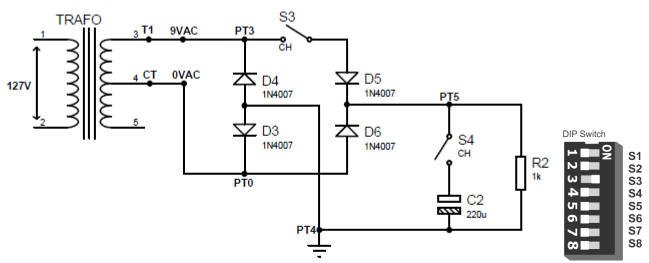
\includegraphics[width=.7\textwidth]{RetificadorPonte.png}
\caption{Circuito equivalente do retificador de onda completa tipo ponte.}
\label{circ2}
\end{figure}

Para realizar a filtragem capacitiva da tensão na saída do retificador da Figura \ref{circ2}, posicione as chaves S3 e S4 do \textit{DIP Switch} na posição fechada (ON) e mantenha as demais abertas. Desta forma, o capacitor C2 da Figura \ref{circ2} é inserido na saída do retificador.

\subsection*{Questionário}

\begin{enumerate}
\setcounter{enumi}{5}

\item (1,0 pontos) Com o auxílio de um osciloscópio, meça a tensão de saída do retificador tipo ponte (Figura \ref{circ2}) \textbf{sem} o filtro capacitivo. Esboce a forma de onda observada e meça os valores de pico a pico, eficaz, médio, o período e a frequência.

\begin{figure}[!h]
	\centering
	\begin{tikzpicture}
		\draw[step=.5cm,gray,very thin] (0,0) grid (6,4);	
	\end{tikzpicture}
\end{figure}

\begin{table}[!h]
\centering
%\caption{Tensão de saída do retificador de onda completa com derivação central.}
\begin{tabular}{|c|c|c|c|c|}
\hline
Valor & Acoplamento CC & Acoplamento CA & Período & Frequência\\\hline
Pico-pico & & & & \\\cline{1-3}
Eficaz & & & & \\\cline{1-3}
Médio & & & & \\\hline
\end{tabular}
\end{table}

\item (1,0 pontos) Com o auxílio de um osciloscópio, e utilizando o \textbf{Acoplamento CC}, meça a tensão de saída do retificador tipo ponte (Figura \ref{circ2}) \textbf{com} o filtro capacitivo. Em seguida, responda as questões a seguir:

\begin{enumerate}
\item A forma de onda deixou de ser pulsante?
\item Qual o novo valor médio da tensão de saída?
\end{enumerate}

\end{enumerate}

\end{document}
